\section{Groepen}
\warning{Heap algoritme}

\warning{}
\subsection{Partitionering van de groepselementen in conjugatieklassen}
\subsection{Cykelindices}
Op het examen wordt er gevraagd om de cykelindex van een willekeurige drie dimensionele veelhoek te bepalen. Daarna wordt er gevraagd om het aantal configuraties te bepalen waarbij een X aantal kleuren Y maal gebruikt worden.

Op deze vraag moet de AntiView gebruikt worden die standaard al open staat op het examen met de figuur. Dit programma toont default de symmetrie en rotatie-assen niet. Zonder dit hulpmiddel is deze vraag haast onmogelijk. Je kan de assen tonen door op de knop 'Y' te drukken op het toetsenbord. In de voorbeelden gebruiken we een kubus. Je kan deze figuur ook bekomen door het programma AntiView via de commandolijn op te starten met als argument \texttt{cube}.

\begin{center}
 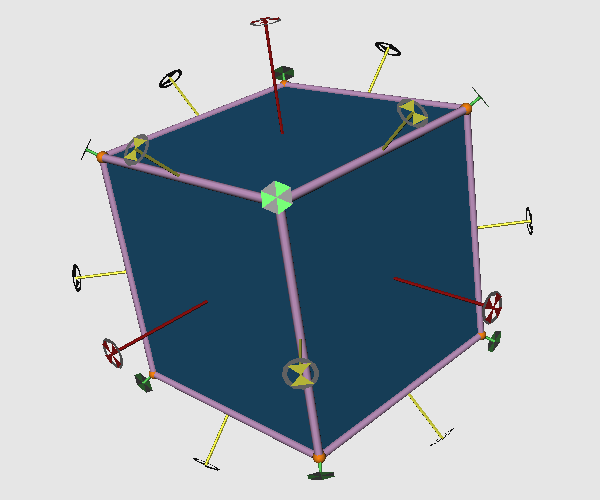
\includegraphics[width=\linewidth]{antiview_cube_1}
\end{center}

Normaal zie je 3 soorten assen verschijnen: rode, gele en groene. Elke kleur heeft zijn eigen betekenis.
\begin{itemize}
 \item \textbf{Rood}:
 \item \textbf{Geel}:
 \item \textbf{Groen}:
\end{itemize}
